\section{Prolog Optimization Engine}

To integrate all stages of the optimization pipeline, a coordinating class is used to drive the complete transformation process. This class coordinates the end-to-end interaction with Prolog, from loading logic rules to returning reconstructed intermediate representation (IR) nodes. Each Prolog-based optimization is encapsulated within its own Java class. For example, optimizations targeting canonicalization rules for the \texttt{AddNode} are implemented in the \texttt{AddNodeProlog} class, while conditional elimination optimizations are handled by the \texttt{ConditionalEliminationProlog} class. This modular design promotes separation of concerns, allowing each optimization to define the specific IR node types it operates on, the logic for translating IR nodes into Prolog terms, and the structure of the Prolog queries it executes.
Stateless optimizations, such as canonicalization and loop-invariant reassociation, use a singleton class instance to avoid reloading rules and reduce startup overhead. In contrast, stateful optimizations require a fresh instance for each execution, as they may modify or depend on internal state during processing.

The coordinator leverages the \texttt{Projog} library, a Java-based Prolog interpreter, to allow seamless query execution and rule evaluation within the Java environment.
Projog is used as the embedded Prolog engine due to its seamless compatibility with Java and support for custom rule definitions. Unlike traditional native Prolog runtimes (such as SWI-Prolog) that run as separate processes, Projog runs entirely within the Java Virtual Machine as a library (delivered via a JAR file). This means it does not require starting an external Prolog process or communicating between separate processes using interprocess communication (IPC) mechanisms like sockets or standard input/output streams. Additionally, there is no need to install or manage an external Prolog runtime on the system. This tight integration enables Prolog queries to be invoked directly within the GraalVM infrastructure as part of the compilation pipeline, simplifying deployment and improving performance by avoiding overhead associated with external processes.

Each optimization class follows a common execution pipeline:
\begin{enumerate}
    \item \textbf{Rule Loading:} At initialization, the engine loads a \texttt{.pl} file containing Prolog rules into the instance's knowledge base. These rules define the conditions and transformations associated with a particular IR pattern.
    
    \item \textbf{IR-to-Prolog Translation:} The IR node to be optimized is recursively translated into a corresponding Prolog term.

    \item \textbf{Fact Generation (Optional):} Before constructing the query, additional facts representing relevant structural or contextual information are dynamically asserted into the knowledge base.
    
    This step is necessary because the original nested IR graph structure is difficult to analyze directly for conditional elimination. For example, in conditional elimination, each \texttt{if} node has a fact asserted to record its position in the dominator tree, which helps the query reason about control flow order.

    \item \textbf{Query Construction:} Construct a query with the translated Prolog term.
    
    \item \textbf{Query Execution:} The query is submitted to the Projog engine. If a matching rule is found, the engine binds \texttt{ResultTerm} to a Prolog term that encodes the optimized form.
    
    \item \textbf{Result Parsing:} The Prolog term returned as the result is parsed using the \texttt{PrologResultParser}. This converts it back into a Java representation suitable for IR construction.
    
    \item \textbf{IR Reconstruction:} Finally, the parsed representation is transformed into a new GraalVM IR node using the visitor-based reconstruction mechanism described earlier.
\end{enumerate}

\textbf{End-to-End Optimization Example}

The example illustrated in Figure~\ref{fig:diagram} demonstrates the full optimization pipeline for a canonicalization rule applied to an addition operation. Starting from the IR graph representation of the original code, the process begins by translating the relevant IR subtrees into Prolog terms and constructing a query (step 1). The constructed query expresses a search for a canonicalized form of an addition operation. It takes two arguments: the first argument describes the addition operation and its operands in detail, while the second argument is a variable that will hold the result returned by the Prolog engine. The first operand of the \texttt{addnode} is a \texttt{subnode} represented by node 5, and the second operand is a parameter node 3 representing the variable \texttt{y}. The \texttt{subnode} itself has two operands: node 2, representing the variable \texttt{x}, and node 3, representing \texttt{y}. The Prolog query is then executed, and the engine returns a result, \texttt{lookup(2)}, indicating that the expression simplifies to an existing node, node \texttt{x} (step 2). This result is parsed into an internal representation by the Prolog result parser (step 3), which is subsequently used to reconstruct the corresponding GraalVM IR node by retrieving node ID 2 from the graph (step 4). The final output reflects the optimized method, where the original expression \texttt{(x - y) + y} is simplified to just \texttt{x}. This sequence demonstrates how the system translates, queries, parses, and reconstructs optimized IR seamlessly within the compilation pipeline.

\begin{figure}
    \centering
    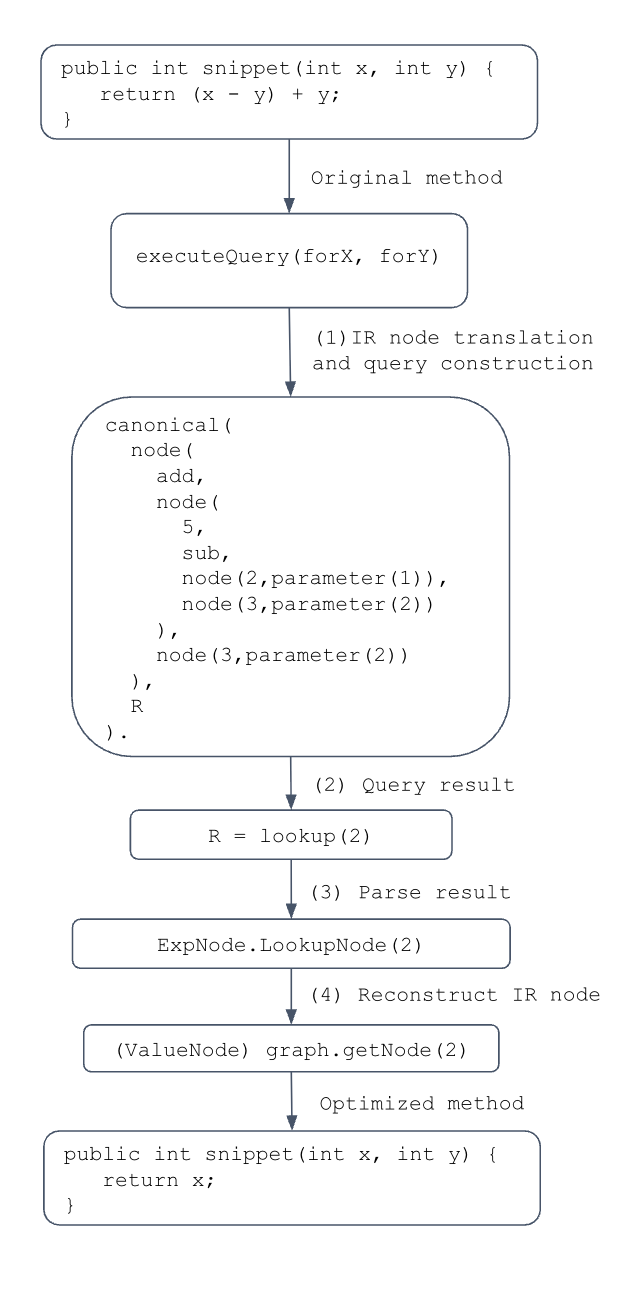
\includegraphics[width=0.5\textwidth]{./Packages/diagram.png}
    \caption{Prolog-Based Optimization Workflow}
    \label{fig:diagram}
\end{figure}